\documentclass[mathserif,11pt,handout]{beamer}

\usepackage{url,verbatim,natbib}
\usepackage[english]{babel}
\usepackage{amsmath, mathabx}
\usepackage{dsfont, ulem}
\usepackage{tikz}
\usepackage{xparse}
\usepackage{pgfpages}
\pgfpagesuselayout{4 on 1}[a4paper, border shrink=5mm, landscape]
\newtheorem{proposition}[theorem]{Proposition}

\usepackage[headheight=22pt]{beamerthemeboxes}
\usepackage{graphicx}
\beamertemplatenavigationsymbolsempty 
\setbeamercovered{transparent}
\usepackage{centernot}

\setbeamertemplate{itemize item}{$\bullet$} 
\setbeamercolor{title}{fg=uio}
\setbeamertemplate{sections/subsections in toc}[ball unnumbered]
\setbeamercolor{section in toc}{fg=uio,bg=white}
\setbeamercolor{subsection in toc}{fg=uio,bg=white}
\setbeamercolor{result}{fg=black, bg=yellow}
\newcommand{\dotsim}{\stackrel{\cdot}{\sim}}
\newcommand{\interi}{{\rm Z}\negthinspace\negthinspace {\rm Z}}
\newcommand{\reali}{{\rm I}\negthinspace {\rm R}}
\newcommand{\naturali}{{\rm I}\negthinspace {\rm N}}
\newcommand{\sign}{\mathop{\rm sgn}\nolimits}
\newcommand{\sgn}{\mathop{\mathrm{sgn}}}
\definecolor{redve}{rgb}{0.604,0.008,0.00}
\definecolor{lmu}{rgb}{0.188,0.522,0.306}
\definecolor{uio}{rgb}{0.847,0.118,0.02}

\def\R{{\rm I\!R}}
\def\P{{\rm Pr}}
\def\Real{{\rm I\!R}}
\def\T{{\footnotesize {^{_{\sf T}}}}}
\def\tr{{\rm tr}}
\def\diag{{\rm diag}}

\NewDocumentCommand\DownArrow{O{2.0ex} O{black}}{%
   \mathrel{\tikz[baseline] \draw [<-, line width=0.5pt, #2] (0,0) -- ++(0,#1);}
}

\useframetitletemplate{% 
\begin{centering} 
\begin{small} \structure{\textcolor{uio} \insertframetitle {\insertframesubtitle}}
\end{small}

\end{centering} 
}

\addheadboxtemplate{\color[rgb]{1,1,1}}{\color{uio} \underline{{\hspace{5pt}\includegraphics[scale=0.06]{../../../../support/uio_logo_eng} \hspace{0.265\paperwidth}\color{black} \tiny  STK-IN4300 - Statistical Learning Methods in Data Science} \hspace{5pt}}}

%\bfseries{\insertsection}

\addfootboxtemplate{\color[rgb]{1,1,1}}{\color{black} \tiny \quad  
STK-IN4300: lecture 5
  \hfill \tiny \insertframenumber / \inserttotalframenumber \hspace{5pt}}

  
\title{STK-IN4300 \\ Statistical Learning Methods in Data Science}
\author{Riccardo De Bin} 
\institute{debin@math.uio.no} 
\date{}


\begin{document}
\setbeamercolor{bgr}{fg=black,bg=uio}

{
\setbeamertemplate{headline}{}
\frame{
\vspace{-2cm}
\begin{beamercolorbox}[sep=-2.2em,wd=5cm,colsep=0.5pt,ht=4.25ex,dp=3ex,left]{postit}
\includegraphics[scale=0.06]{../../../../support/uio_logo_eng}
\end{beamercolorbox}
\vspace{0.365cm}
\noindent\makebox[\linewidth]{\color{uio} \rule{\paperwidth}{0.4pt}}
\vspace{2.5cm}
\titlepage
}
}

\frame{\frametitle{Outline of the lecture}
\tableofcontents
}


\section{Shrinkage Methods}

\frame{\frametitle{Shrinkage Methods: }
\framesubtitle{ridge regression and PCR}
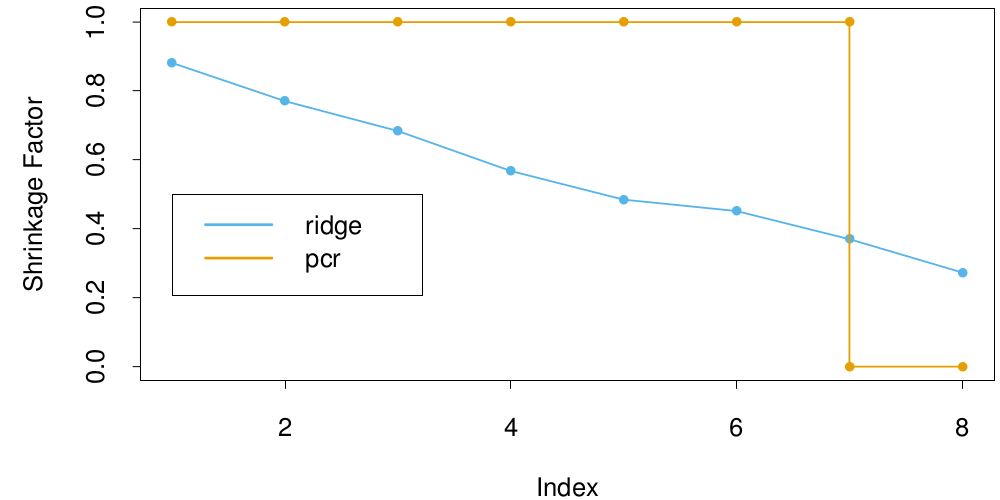
\includegraphics[width=\textwidth]{pcr}
}


\frame{\frametitle{Shrinkage Methods: }
\framesubtitle{bias and variance}
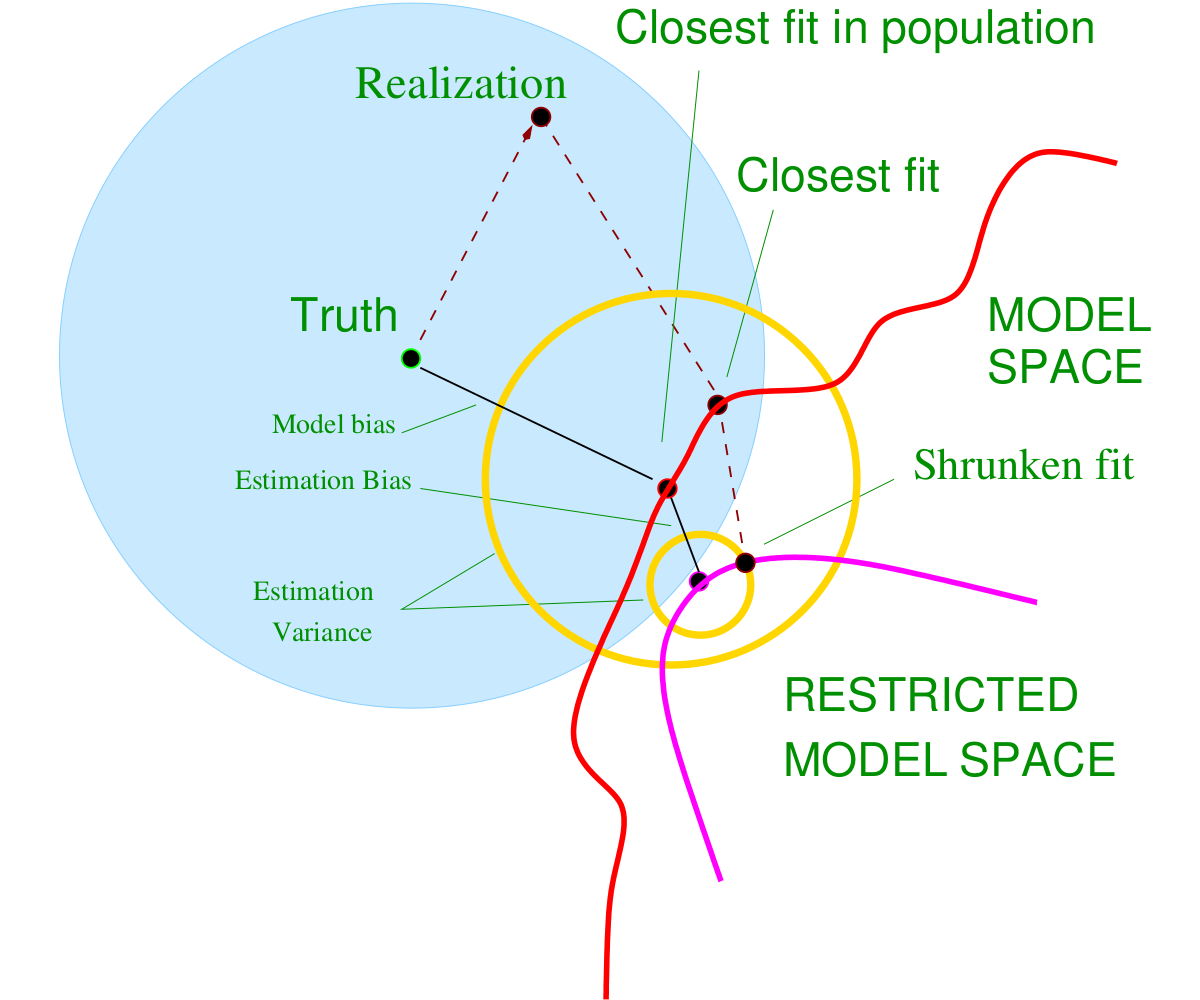
\includegraphics[width=\textwidth]{biasModel}
}


\subsection{Lasso}

\frame{\frametitle{Lasso: }
\framesubtitle{Least Absolute Shrinkage and Selection Operator}
Lasso is \textcolor{uio}{similar} to ridge regression, with an \textcolor{uio}{$L_1$ penalty} instead of the $L_2$ one,
$$
\sum_{i = 1}^N (y_i - \beta_0 - \sum_{j=1}^p \beta_j x_{ij})^2,
$$
subject to $\sum_{j=1}^p |\beta_j| \leq t$.

\hspace{2pt}

Or, in the equivalent Lagrangian form,
$$
\hat{\beta}_\text{lasso}(\lambda) = \text{argmin}_\beta \left\{\sum_{i = 1}^N (y_i - \beta_0 - \sum_{j=1}^p \beta_j x_{ij})^2 + \lambda \sum_{j=1}^p |\beta_j|\right\}.
$$
\begin{itemize}
\item $X$ must be \textcolor{uio}{standardized};
\item $\beta_0$ is again \textcolor{uio}{not considered} in the penalty term.
\end{itemize}
}


\frame{\frametitle{Lasso: }
\framesubtitle{remarks}
Due to the structure of the $L_1$ norm;
\begin{itemize}
  \item some estimates are \textcolor{uio}{forced to be 0} (variable selection);
  \item \textcolor{uio}{no close form} for the estimator.
  \item[]
\end{itemize}

From a Bayesian prospective:
\begin{itemize}
  \item $\hat{\beta}_\text{lasso}(\lambda)$ as the posterior mode estimate.
  \item $\beta \sim Laplace(0,\tau^2)$;
  \item for more details, see \cite{ParkCasella2008}.
  \item[]
\end{itemize}

Extreme situations:
\begin{itemize}
\item $\lambda \rightarrow 0$, $\hat{\beta}_\text{lasso}(\lambda) \rightarrow \hat{\beta}_\text{OLS}$;
\item $\lambda \rightarrow \infty$, $\hat{\beta}_\text{lasso}(\lambda) \rightarrow 0$.
\end{itemize}
}


\frame{\frametitle{Lasso: }
\framesubtitle{constrained estimation}
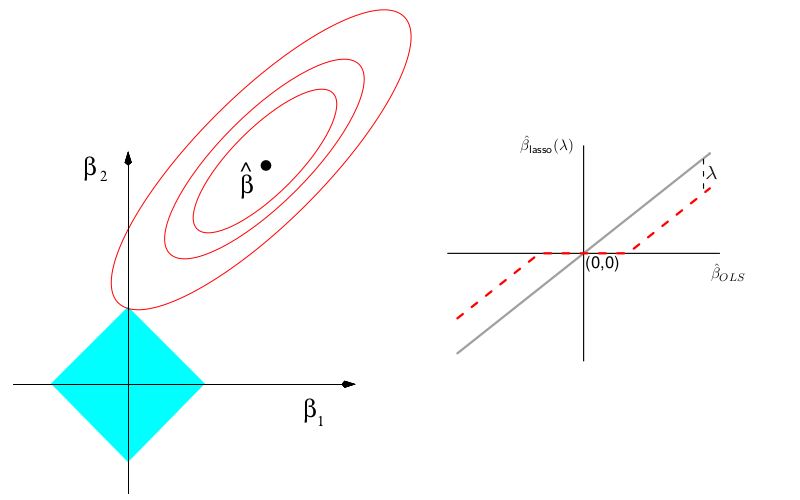
\includegraphics[width=\textwidth]{lasso_con}
}


\frame{\frametitle{Lasso: }
\framesubtitle{shrinkage}
\centering
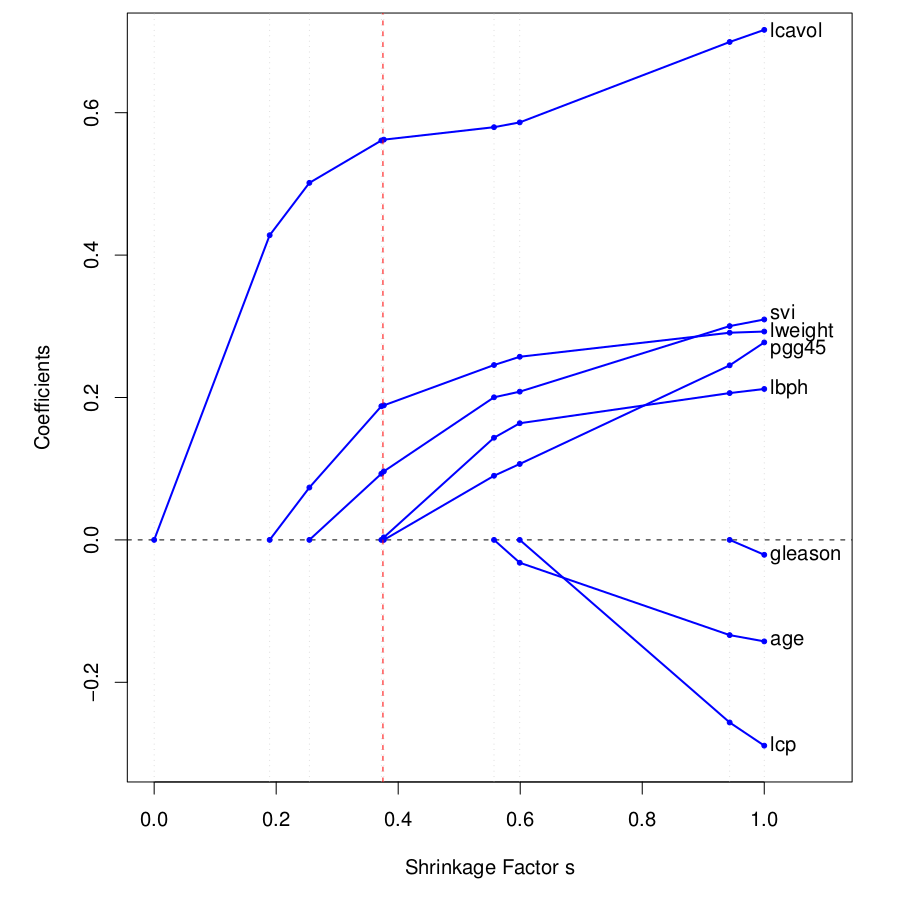
\includegraphics[width=0.72\textwidth]{lasso}
}


\frame{\frametitle{Lasso: }
\framesubtitle{generalized linear models}
Lasso (and ridge r.) can be used with \textcolor{uio}{any linear regression} model;
\begin{itemize}
\item e.g., logistic regression.
\item[]
\end{itemize}
In \textcolor{uio}{logistic regression}, the lasso solution is the maximizer of
$$
\text{max}_{\beta_0, \beta} \left\{\sum_{i = 1}^N \left[y_i(\beta_0 + \beta^T x_i) -\log(1+e^{\beta_0 + \beta^T x_i})\right] - \lambda \sum_{j=1}^p |\beta_j|\right\}.
$$
Note:
\begin{itemize}
\item penalized logistic regression can be applied to problems with \textcolor{uio}{high-dimensional data} (see Section 18.4).
\end{itemize}
}


\subsection{Comparison of Shrinkage Methods}

\frame{\frametitle{Comparison of Shrinkage Methods: }
\framesubtitle{coefficient profiles}
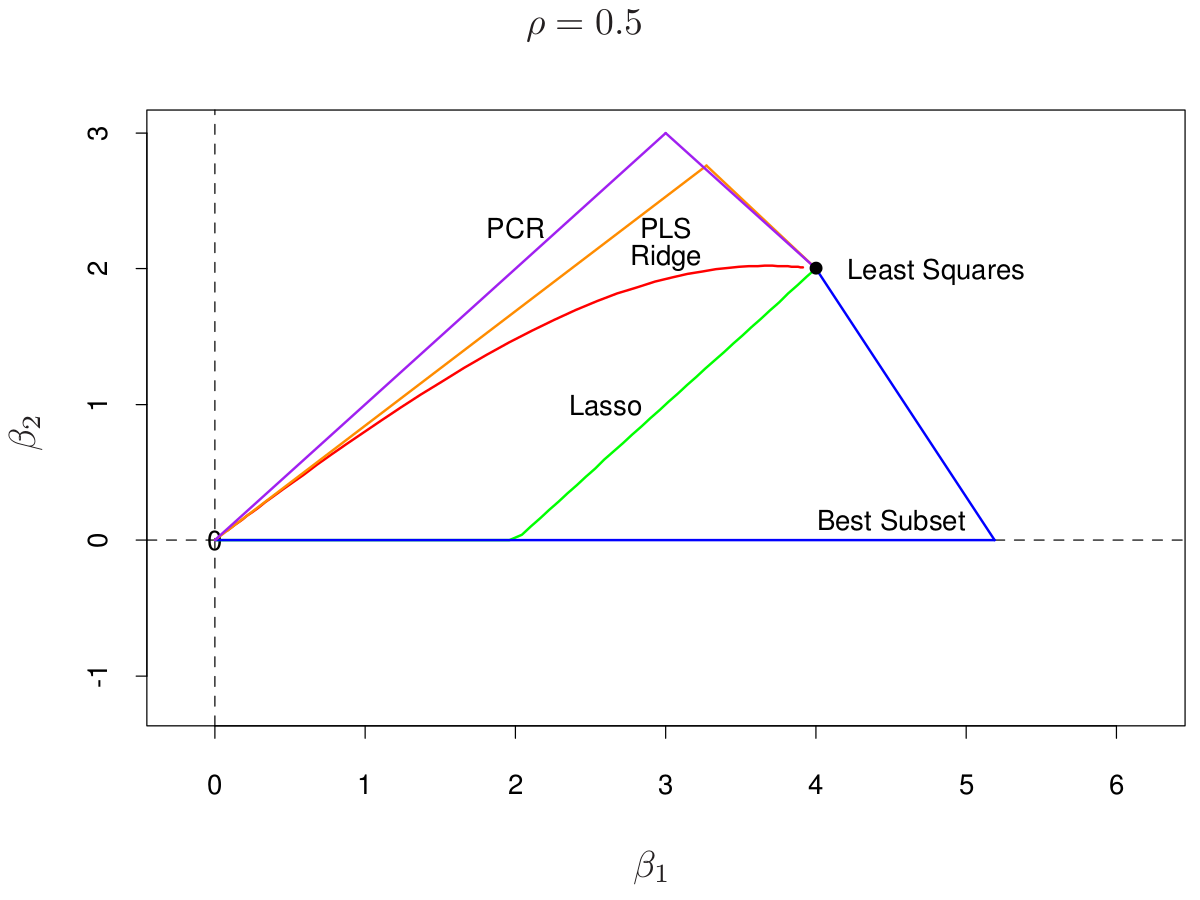
\includegraphics[width=0.92\textwidth]{path_1}
}


\frame{\frametitle{Comparison of Shrinkage Methods: }
\framesubtitle{coefficient profiles}
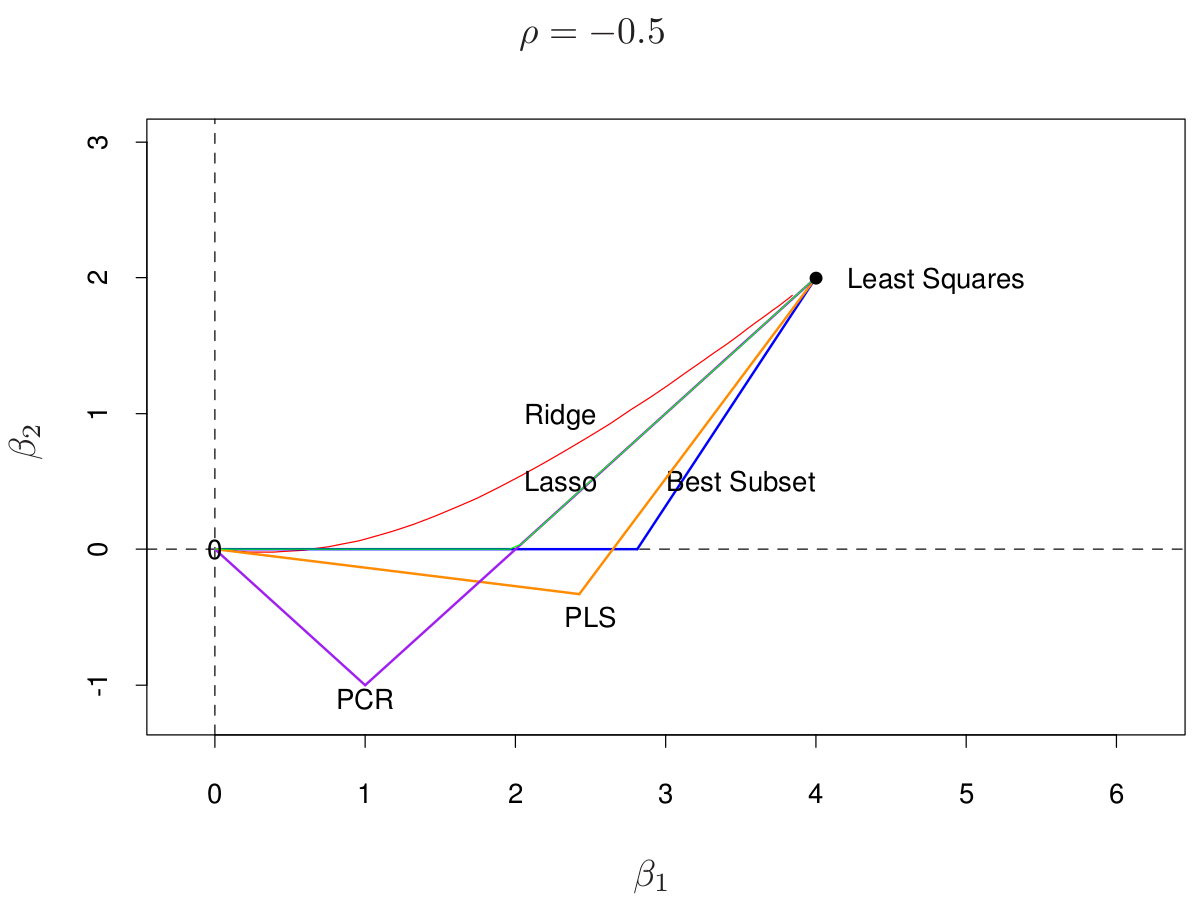
\includegraphics[width=0.92\textwidth]{path_2}
}


\frame{\frametitle{Comparison of Shrinkage Methods: }
\framesubtitle{coefficient profiles}
\centering
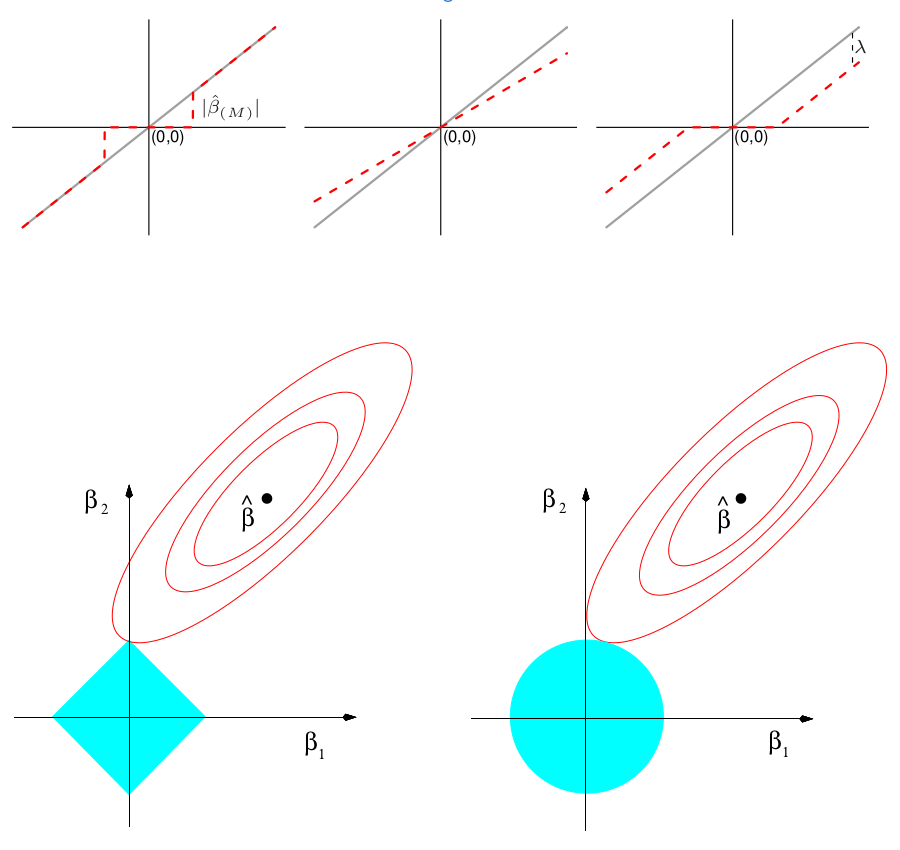
\includegraphics[width=0.72\textwidth]{shrinkage}
}


\subsection{More on Lasso and Related Path Algorithms}

\frame{\frametitle{More on Lasso and Related Path Algorithms: }
\framesubtitle{generalization}
\textcolor{uio}{Generalization} including lasso and ridge r.\ $\rightarrow$ {\bf \uline{bridge regression}}:
$$
\tilde{\beta}(\lambda) = \text{argmin}_\beta \left\{\sum_{i = 1}^N (y_i - \beta_0 - \sum_{j=1}^p \beta_j x_{ij})^2 + \lambda \sum_{j=1}^p |\beta_j|^q\right\}, q\geq0.
$$
Where:
\begin{itemize}
\item $q=0$ $\rightarrow$ \textcolor{uio}{best subset selection};
\item $q=1$ $\rightarrow$ \textcolor{uio}{lasso};
\item $q=2$ $\rightarrow$ \textcolor{uio}{ridge regression}.
\end{itemize}
}


\frame{\frametitle{More on Lasso and Related Path Algorithms: }
\framesubtitle{generalization}
Note that:
\begin{itemize}
\item $0 < q \leq 1$ $\rightarrow$ \textcolor{uio}{non differentiable};
\item $1 < q < 2$ $\rightarrow$ compromise between lasso and ridge (but \textcolor{white}{makespaceoii} differentiable $\Rightarrow$ \textcolor{uio}{no variable selection} property).
\item $q$ defines the \textcolor{uio}{shape} of the constrain area:
\end{itemize}
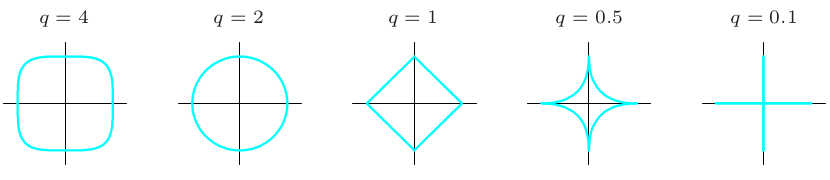
\includegraphics[width=\textwidth]{fig3_12}
\begin{itemize}
\item $q$ could be estimated from the data (\textcolor{uio}{tuning parameter});
\item in practice does \textcolor{uio}{not work} well (variance).
\end{itemize}
}


\frame{\frametitle{More on Lasso and Related Path Algorithms: }
\framesubtitle{elastic net}
Different \textcolor{uio}{compromise} lasso / ridge regression: {\bf \underline{elastic net}}
\small
$$
\tilde{\beta}(\lambda) = \text{argmin}_\beta \left\{\sum_{i = 1}^N (y_i - \beta_0 - \sum_{j=1}^p \beta_j x_{ij})^2 + \lambda \sum_{j=1}^p \left(\alpha |\beta_j| + (1-\alpha) \beta_j^2 \right)\right\}.
$$
Idea:
\begin{itemize}
\item \textcolor{uio}{$L_1$} penalty takes care of \textcolor{uio}{variable selection};
\item \textcolor{uio}{$L_2$} penalty helps in correctly \textcolor{uio}{handling correlation};
\item $\alpha$ defines \textcolor{uio}{how much} $L_1$ and $L_2$ penalty should be used:
\begin{itemize}
\item it is a \textcolor{uio}{tuning parameter}, must be found in addition to  $\lambda$;
\item a grid search is \textcolor{uio}{discouraged};
\item in real experiments, \textcolor{uio}{often} very close to 0 or 1.
\end{itemize}
\end{itemize}
}


\frame{\frametitle{More on Lasso and Related Path Algorithms: }
\framesubtitle{elastic net}
Comparing the bridge regression and the elastic net,
\begin{center}
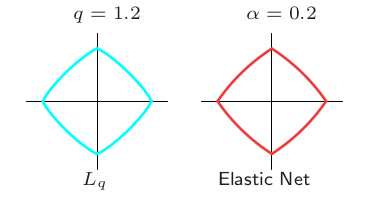
\includegraphics[width=0.8\textwidth]{fig3_13_small}
\end{center}
\begin{itemize}
\item they look \textcolor{uio}{very similar};
\item huge difference due to \textcolor{uio}{differentiability} (variable selection).
\end{itemize}
}


\frame{\frametitle{More on Lasso and Related Path Algorithms: }
\framesubtitle{Least Angle Regression}
The \textcolor{uio}{Least Angle Regression} ({\bf \underline{LAR}}):
\begin{itemize}
\item can be viewed as a \textcolor{uio}{``democratic''} version of the forward selection;
\item \textcolor{uio}{add} sequentially a \textcolor{uio}{new} predictors into the model
\begin{itemize}
\item only \textcolor{uio}{``as much as it deserves''};
\end{itemize}
\item eventually reaches the least square estimation;
\item strongly connected with lasso;
\begin{itemize}
\item lasso can be seen as a \textcolor{uio}{special case} of LAR;
\item LAR is often used to fit lasso models.
\end{itemize}
\end{itemize}}


\frame{\frametitle{More on Lasso and Related Path Algorithms: }
\framesubtitle{LAR}
Least Angle Regression:
\begin{enumerate}
\item \textcolor{uio}{Standardize} the predictors (mean zero, unit norm). Initialize:
\begin{itemize}
  \item residuals $r = y - \bar{y}$
  \item regression coefficient estimates $\beta_1 = \dots = \beta_p = 0$;
\end{itemize}
\item find the predictor $x_j$ \textcolor{uio}{most correlated} with $r$;
\item move $\hat{\beta}_j$ towards its \textcolor{uio}{least-squares coefficient} $\langle x_j, r \rangle$,
\begin{itemize}
\item \textcolor{uio}{until} for $k\neq j$, $\text{corr}(x_k, r) = \text{corr}(x_j, r)$.
\end{itemize}
\item add $x_k$ in the \textcolor{uio}{active list} and update \textcolor{uio}{both} $\hat{\beta}_j$ and $\hat{\beta}_k$:
\begin{itemize}
\item towards their joint least squares coefficient;
\item until $x_l$ has as much correlation with the current residual;
\end{itemize}
\item continue until \textcolor{uio}{all} $p$ predictors have been entered.
\end{enumerate}
}


\frame{\frametitle{More on Lasso and Related Path Algorithms: }
\framesubtitle{comparison}
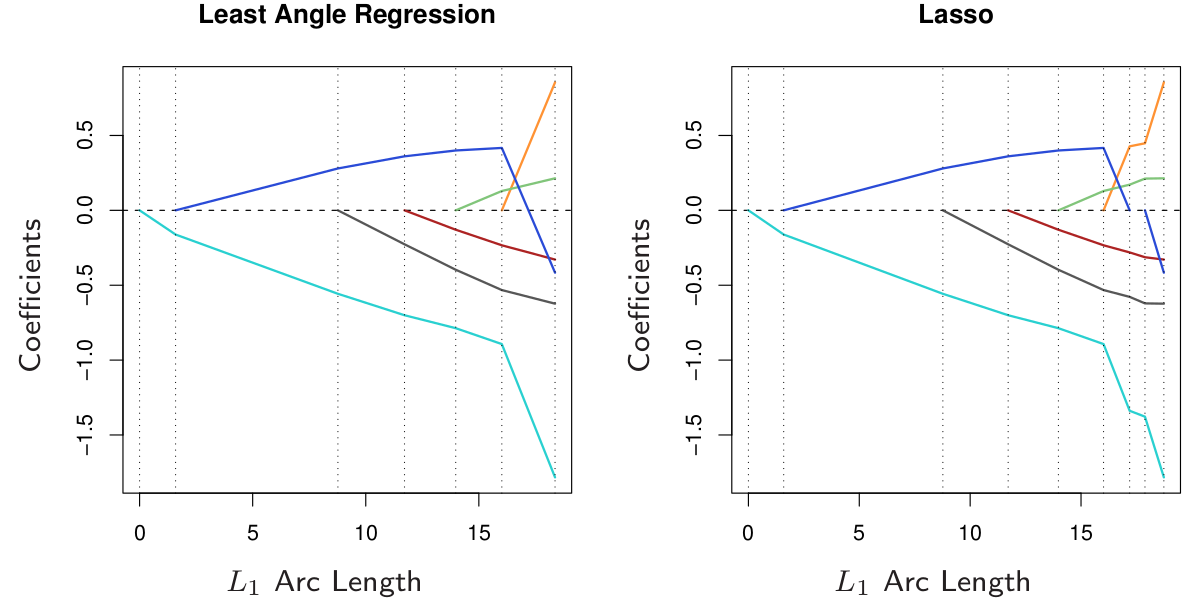
\includegraphics[width=\textwidth]{lar}
}


\frame{\frametitle{More on Lasso and Related Path Algorithms: }
\framesubtitle{overfit}
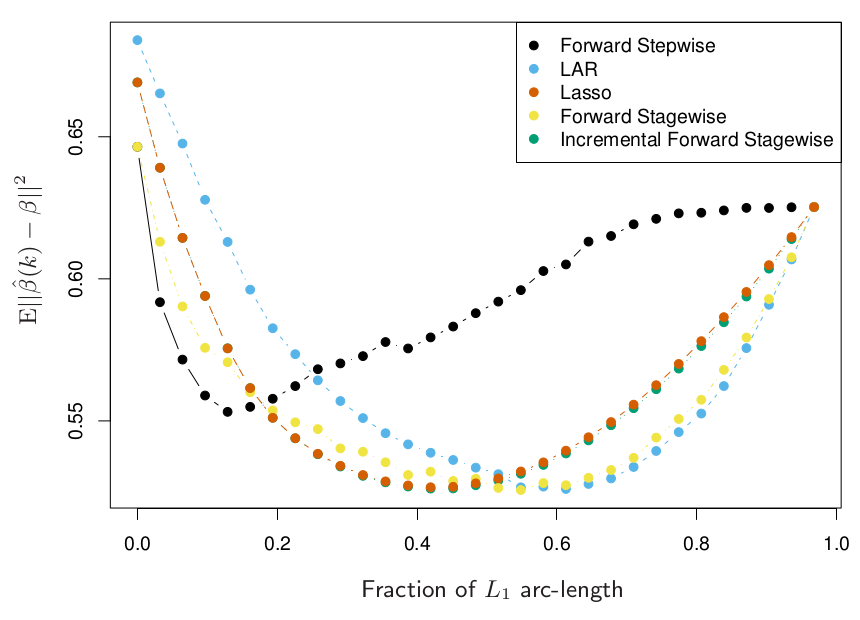
\includegraphics[width=\textwidth]{fig3_16}
}


\frame{\frametitle{More on Lasso and Related Path Algorithms: }
\framesubtitle{other shrinkage methods}
{\bf \uline{Group Lasso}}

Sometimes predictors \textcolor{uio}{belong} to the \textcolor{uio}{same group}:
\begin{itemize}
\item genes that belong to the same molecular pathway;
\item dummy variables from the same categorical variable \dots
\end{itemize}
Suppose the $p$ predictors are grouped in $L$ groups, group lasso minimizes
$$
\text{min}_\beta \left\{||(y - \beta_0\vec{1} - \sum_{\ell=1}^L X_{\ell}\beta_\ell ||_2^2 + \lambda \sum_{\ell=1}^L \sqrt{p_\ell} ||\beta_j||_2 \right\},
$$
where:
\begin{itemize}
\item $\sqrt{p_\ell}$ accounts for the \textcolor{uio}{group sizes};
\item $||\cdot||$ denotes the (not squared) Euclidean norm
\begin{itemize}
\item it is 0 $\Leftarrow$ all its component are 0;
\end{itemize}
\item \textcolor{uio}{sparsity} is encouraged at \textcolor{uio}{both} group and individual levels.
\end{itemize}
}


\frame{\frametitle{More on Lasso and Related Path Algorithms: }
\framesubtitle{other shrinkage methods}
{\bf \uline{Non-negative garrote}}

The idea of lasso originates from the \textcolor{uio}{non-negative garrote},
$$
\hat{\beta}_\text{garrote} = \text{argmin}_\beta \sum_{i=1}^N (y_i - \beta_0 - \sum_{j=1}^p c_j\beta_j x_{ij})^2,
$$
subject to
$$
c_j \geq 0 \text{ and } \sum_j c_j \leq t.
$$
Non-negative garrote \textcolor{uio}{starts} with \textcolor{uio}{OLS} estimates and \textcolor{uio}{shrinks} them:
\begin{itemize}
 \item by \textcolor{uio}{non-negative factors};
 \item the sum of the non-negative factor is \textcolor{uio}{constrained};
 \item for more information see \cite{Breiman1995}.
\end{itemize}
}


\frame{\frametitle{More on Lasso and Related Path Algorithms: }
\framesubtitle{other shrinkage methods}
In the case of \textcolor{uio}{orthogonal} design ($X^TX=I_N$),
$$
c_j(\lambda) = \left(1-\frac{\lambda}{\hat{\beta}_j^{OLS}}\right),
$$
where $\lambda$ is a tuning parameter (related to $t$).

\vspace{12pt}

Note that the solution depends on $\hat{\beta}_\text{OLS}$:
\begin{itemize}
\item \textcolor{uio}{cannot} be applied in $p >> N$ problems;
\item may be a problem when $\hat{\beta}_\text{OLS}$ behaves \textcolor{uio}{poorly};
\item has the \textcolor{uio}{oracle properties} \citep{YuanLin2006} $\leftarrow$ see soon.
\end{itemize}
}


\frame{\frametitle{More on Lasso and Related Path Algorithms: }
\framesubtitle{other shrinkage methods}
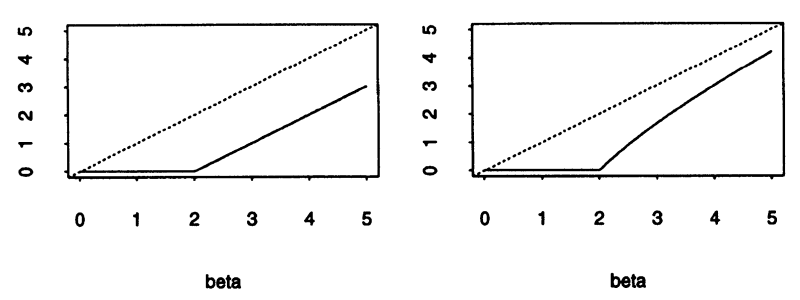
\includegraphics[width=\textwidth]{garrote}

Comparison between lasso (left) and non-negative garrote (right).

\vspace{40pt}

\citep[picture from][]{Tibshirani1996}
}



\frame{\frametitle{More on Lasso and Related Path Algorithms: }
\framesubtitle{the oracle property}
Let:
\begin{itemize}
\item $\mathcal{A}:=\{j:\beta_j\neq0\}$ be the set of the \textcolor{uio}{true relevant coefficients};
\item $\delta$ be a \textcolor{uio}{fitting procedure} (lasso, non-negative garrote, \dots);
\item $\hat{\beta}(\delta)$ the coefficient \textcolor{uio}{estimator} of the procedure $\delta$.
\item[]
\end{itemize}

We would like that $\delta$:
\begin{itemize}
\item[(a)] \textcolor{uio}{identifies} the right subset model, $\{j:\hat{\beta}(\delta)\neq 0\} = \mathcal{A}$;
\item[(b)] has the \textcolor{uio}{optimal estimation rate}, $\sqrt{n}(\hat{\beta}(\delta)_\mathcal{A} - \beta_\mathcal{A}) \xrightarrow{d} N(0,\Sigma)$, where $\Sigma$ is the covariance matrix for the true subset model.
\item[]
\end{itemize}

If $\delta$ satisfies (a) and (b), it is called an \textcolor{uio}{oracle procedure}.
}


\frame{\frametitle{More on Lasso and Related Path Algorithms: }
\framesubtitle{lasso and oracle property}
Consider the following setup \citep{KnightFu2000}:
\begin{itemize}
\item $y_i = x_i\beta + \epsilon_i$, with $\epsilon_i$ i.i.d.\ r.v.\ with mean 0 and variance $\sigma^2$;
\item $n^{-1} X^TX \rightarrow C$, where $C$ is a positive definite matrix;
\item suppose w.l.g.\ that $\mathcal{A} = \{1,2,\dots,p_0\}$, $p_0<p$;
\item $C=\left[\begin{array}{cc}
 C_{11} & C_{12} \\
 C_{21} & C_{22} \\
\end{array}\right]$, with $C_{11}$ a $p_0\times p_0$ matrix;
\item $\hat{\mathcal{A}} = \{j:\hat{\beta}_j^\text{lasso}(\lambda) \neq 0\} $
\end{itemize}}


\frame{\frametitle{More on Lasso and Related Path Algorithms: }
\framesubtitle{lasso and oracle property}
\cite{KnightFu2000} demonstrated the following two lemmas:
\begin{lemma}[1]
If $\lambda/n\rightarrow \lambda_0\geq 0$, then $\hat{\beta}^\text{lasso}(\lambda)\xrightarrow{p} \text{argmin}_u\, V_1(u)$, where
$$
V_1(u) = (u-\beta)^TC(u-\beta)^T + \lambda_0\sum_{i=1}^p|u_j|.
$$
\end{lemma}

\begin{lemma}[2]
If $\lambda/\sqrt{n}\rightarrow \lambda_0\geq 0$, then $\sqrt{n}(\hat{\beta}^\text{lasso}(\lambda) - \beta) \xrightarrow{d} \text{argmin}_u\, V_2(u)$,
$$
V_2(u) = -2u^TW + u^TCu + \lambda_0\sum_{i=1}^p[u_j\text{sgn}(\beta)\mathds{1}(\beta \neq 0) + |u_j|\mathds{1}(\beta = 0)].
$$
\end{lemma}
}


\frame{\frametitle{More on Lasso and Related Path Algorithms: }
\framesubtitle{lasso and oracle property}
From Lemma (1):
\begin{itemize}
\item \textcolor{uio}{only} $\lambda_0=0$ guarantees consistency.
\end{itemize}

\vspace{12pt}

Lemma (2) states:
\begin{itemize}
\item the lasso estimate is \textcolor{uio}{$\sqrt{n}$-consistent};
\item when $\lambda = O(\sqrt{n})$, $\hat{\mathcal{A}}$ \textcolor{uio}{cannot} be $\mathcal{A}$ with positive probability.
\end{itemize}

\begin{proposition}[1]
If $\lambda/\sqrt{n} \rightarrow \lambda_0 \geq 0$, then $\text{lim sup}_n P[\hat{\mathcal{A}}=\mathcal{A}] \leq c < 1$.
\end{proposition}
For the proof, see \cite{Zou2006}.
}


\frame{\frametitle{More on Lasso and Related Path Algorithms: }
\framesubtitle{lasso and oracle property}
It may be interesting to see what happens in the \textcolor{uio}{intermediate case}, when $\lambda_0 = \infty$, i.e., $\lambda/n \rightarrow 0$ and $\lambda/\sqrt{n} \rightarrow \infty$.

\begin{lemma}[3]
If $\frac{\lambda}{n} \rightarrow 0$ and $\frac{\lambda}{\sqrt{n}} \rightarrow \infty$, then $\frac{n}{\lambda} (\hat{\beta}^\text{lasso}(\lambda) - \beta) \xrightarrow{p} \text{argmin}_u\, V_3(u)$,
$$
V_3(u) = u^TCu + \sum_{i=1}^p[u_j\text{sgn}(\beta)\mathds{1}(\beta \neq 0) + |u_j|\mathds{1}(\beta = 0)].
$$
\end{lemma}
Note:
\begin{itemize}
\item the \textcolor{uio}{convergence} rate of $\hat{\beta}^\text{lasso}(\lambda)$ is \textcolor{uio}{slower} than $\sqrt{n}$;
\item the optimal estimation rate is available \textcolor{uio}{only} when $\lambda = O(\sqrt{n})$, but it leads to \textcolor{uio}{inconsistent} variable selection;
\item for the proof, see \cite{Zou2006}.
\end{itemize}
}



\frame{\frametitle{More on Lasso and Related Path Algorithms: }
\framesubtitle{necessary condition}
Can consistency in variable selection can be achieved by \textcolor{uio}{sacrificing} the rate of convergence in estimation?
\vspace{-12pt}
$$ \downarrow $$
\begin{center}
\vspace{-12pt}
Non necessarily.
\end{center}


It is possible to derive a \textcolor{uio}{necessary condition} for consistency of the lasso variable selection \citep{Zou2006}: 
\begin{theorem}[necessary condition]
Suppose that $\lim_n P[\hat{\mathcal{A}}=\mathcal{A}]=1$. Then there exists some sign vector $s=(s_1,\dots,s_{p_0})^T$, $s_j\in\{-1,1\}$, such that
\begin{equation}\label{cond}
|C_{21}C_{11}^{-1}s|\leq 1.
\end{equation}
The last equation is understood componentwise.
\end{theorem}
}


\frame{\frametitle{More on Lasso and Related Path Algorithms: }
\framesubtitle{necessary condition}
If condition \eqref{cond} \textcolor{uio}{fails} $\Rightarrow$ the lasso variable selection is \textcolor{uio}{inconsistent}.

\begin{corollary}[1]
Suppose that $p_0 = 2m + 1 \geq 3$ and $p = p_0 + 1$, so there is one irrelevant predictor. Let $C_{11}=(1-\rho_1)I + \rho_1J_1$, where $J_1$ is the matrix of 1's, $C_{12} = \rho_2\vec{1}$ and $C_{22}=1$. If $-\frac{1}{p_0-1}<\rho_1<\frac{1}{p_0}$ and $1+(p_0-1\rho_1) < |\rho_2| < \sqrt{(1+(p_0-1)/\rho_1/p_0)}$, then condition \eqref{cond} cannot be satisfied. So the lasso variable selection is inconsistent.
\end{corollary}
}


\frame{\frametitle{More on Lasso and Related Path Algorithms: }
\framesubtitle{Corollary (1)}
\begin{proof}[Proof of Corollary (1)]
Note that
\begin{itemize}
 \item $C_{11}^{-1} = \frac{1}{1-\rho_1}(I - \frac{\rho_1}{1+(p_0-1)\rho_1}J_1)$;
 \item $C_{21}C_{11}^{-1} = \frac{\rho_2}{1+(p_0-1)\rho_1}(\vec{1})^T$.
\end{itemize} 

Therefore $C_{21}C_{11}^{-1}s = \frac{\rho_2}{1+(p_0-1)\rho_1}(\sum_{j=1}^{p_0} s_j)\vec{1}$.

\vspace{12pt}

Then, condition \eqref{cond} becomes $\left|\frac{\rho_2}{1+(p_0-1)\rho_1}\right|\cdot\left|\sum_{j=1}^{p_0} s_j\right| \leq 1$.

\vspace{12pt}

Note that when $p_0$ is a odd number, $|\sum_{j=1}^{p_0} s_j |\geq 1$.

\vspace{12pt}

If $|\frac{\rho_2}{1+(p_0-1)\rho_1}| > 1$, then condition \eqref{cond} cannot be satisfied for any sign vector. The choice of $(\rho_1,\rho_2)$ ensures that $C$ is a positive matrix and $|\frac{\rho_2}{1+(p_0-1)\rho_1}| > 1$.
\end{proof}
}


\frame{\frametitle{More on Lasso and Related Path Algorithms: }
\framesubtitle{other shrinkage methods}
The \textcolor{uio}{Smoothly Clipped Absolute Deviation} ({\bf \underline{SCAD}}) estimator
$$
\hat{\beta}_\text{scad}(\lambda,\alpha) = \text{argmin}_\beta \left\{\frac{1}{2}||y - \beta_0\vec{1} - X\beta||_2^2 + \lambda \sum_{j=1}^p p_j(\beta_j;\lambda,\alpha)\right\},
$$
where
$$
\frac{d\,p_j(\beta_j;\lambda,\alpha)}{d \beta_j} = \lambda\left\{\mathds{1}(|\beta_j|\leq \lambda) + \frac{(\alpha\lambda - |\beta_j|)_+}{(\alpha-1)\lambda}\mathds{1}(|\beta_j| > \lambda) \right\}
$$
for $\alpha > 2$.

\vspace{12pt}
Usually:
\begin{itemize}
\item $\alpha$ is set \textcolor{uio}{equal to 3.7} (based on simulations);
\item $\lambda$ is chosen via \textcolor{uio}{cross-validation}.
\end{itemize}
}


\frame{\frametitle{More on Lasso and Related Path Algorithms: }
\framesubtitle{other shrinkage methods}
The SCAD penalty function:
\begin{itemize}
\item penalizes \textcolor{uio}{less} the \textcolor{uio}{largest} regression coefficient estimates;
\item makes the solution \textcolor{uio}{continuous}. In particular,
\end{itemize}
$$
\hat{\beta}_\text{scad}(\lambda,\alpha) = \left\{\begin{array}{ll}
\text{sgn}(\beta)(|\beta_j|-\lambda)_+ & \text{when } |\beta| \leq 2\lambda\\
\{(\alpha-1)\beta - \text{sgn}(\beta)\alpha\lambda\}/(\alpha-2) & \text{when } 2\lambda < |\beta| \leq \alpha\lambda\\
\beta & \text{when } |\beta| > \alpha\lambda\\ 
\end{array}
\right.
$$

\vspace{12pt}

Note that:
\begin{itemize}
\item $\exists$ an \textcolor{uio}{$\sqrt{n}$-consistent} estimator \citep[][Theorem 1]{FanLi2001};
\item the SCAD estimator $\hat{\beta}_\text{scad}(\lambda,\alpha)$ is an \textcolor{uio}{oracle estimator} \citep[][Theorem 2]{FanLi2001}.
\end{itemize}
}


\frame{\frametitle{More on Lasso and Related Path Algorithms: }
\framesubtitle{other shrinkage methods}
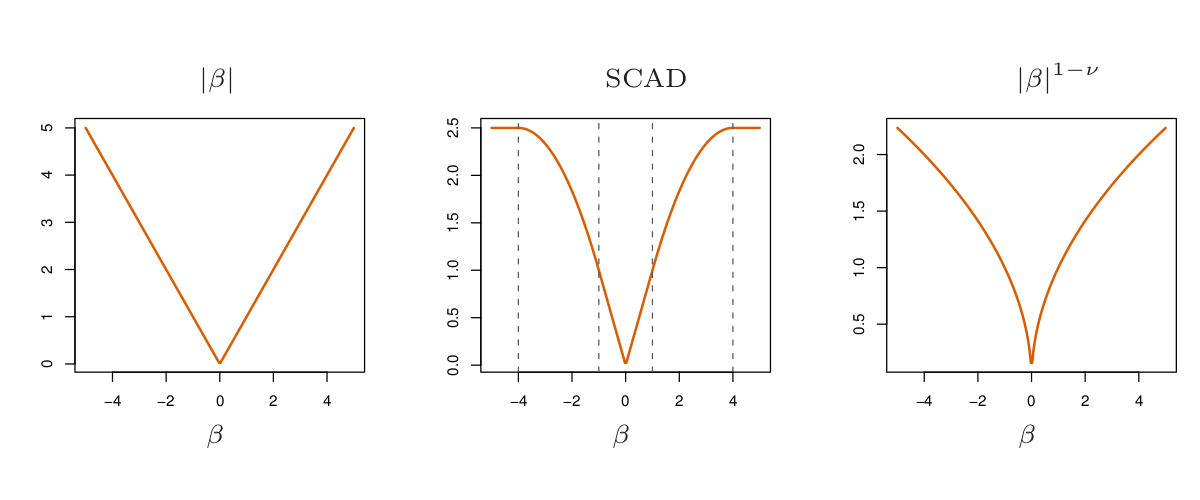
\includegraphics[width=\textwidth]{scad}
}


\frame{\frametitle{More on Lasso and Related Path Algorithms: }
\framesubtitle{other shrinkage methods}
{\bf \uline{Adaptive lasso}}

The \textcolor{uio}{adaptive lasso} is a particular case of the \textcolor{uio}{weighted lasso},
$$
\hat{\beta}_\text{weight}(\lambda) = \text{argmin}_\beta \left\{\sum_{i = 1}^N (y_i - \beta_0 - \sum_{j=1}^p \beta_j x_{ij})^2 + \lambda \sum_{j=1}^p w_j|\beta_j|\right\},
$$
in which \textcolor{uio}{$\hat{w}_j = 1/|\hat{\beta}_\text{OLS}|^\gamma$}.

\vspace{12pt}

Note:
\begin{itemize}
\item it enjoys the \textcolor{uio}{oracle properties} \citep[][Theorem 2]{Zou2006};
\item when $\gamma = 1$, it is \textcolor{uio}{very closely related} to the non-negative garrote (there is an additional sign constrain);
\item \textcolor{uio}{relies on} $\hat{\beta}_\text{OLS}$ $\rightarrow$ sometimes lasso used in a first step;
\item \textcolor{uio}{two-dimensional} tuning parameter.
\end{itemize}
}


\frame{\frametitle{More on Lasso and Related Path Algorithms: }
\framesubtitle{other shrinkage methods}
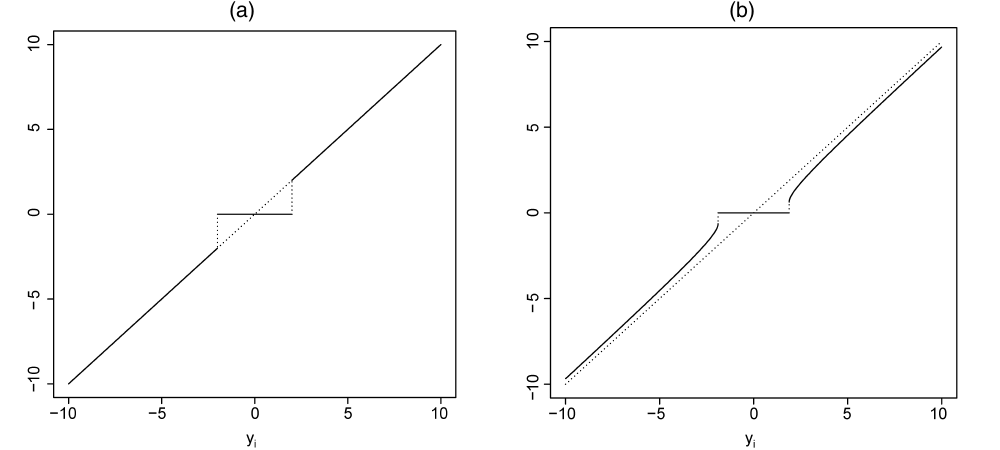
\includegraphics[width=\textwidth]{hard_bridge}
\begin{itemize}
\item[(a)] best subset regression;
\item[(b)] bridge with $\alpha = 0.5$.
\item[]
\end{itemize}
\citep[picture from][]{Zou2006}
}

\frame{\frametitle{More on Lasso and Related Path Algorithms: }
\framesubtitle{other shrinkage methods}
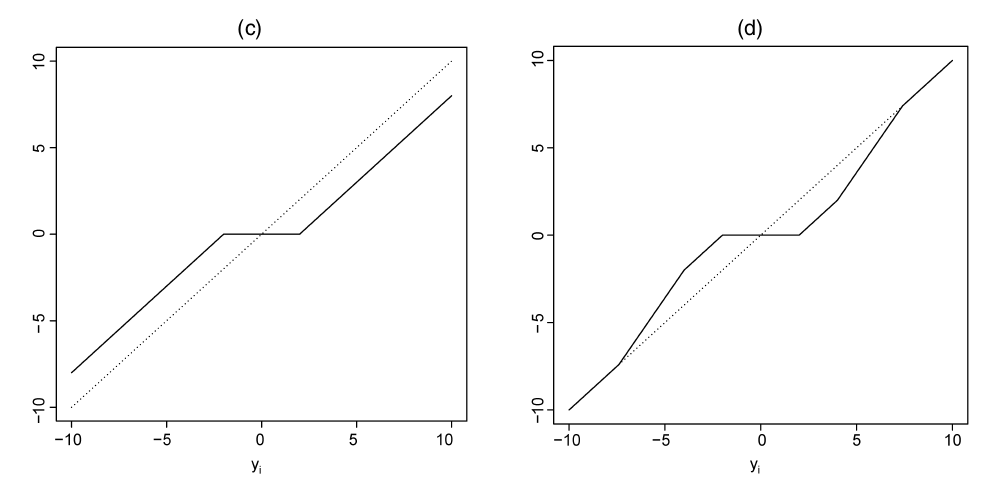
\includegraphics[width=\textwidth]{lasso_scad}
\begin{itemize}
\item[(c)] lasso;
\item[(d)] scad.
\item[]
\end{itemize}
\citep[picture from][]{Zou2006}
}

\frame{\frametitle{More on Lasso and Related Path Algorithms: }
\framesubtitle{other shrinkage methods}
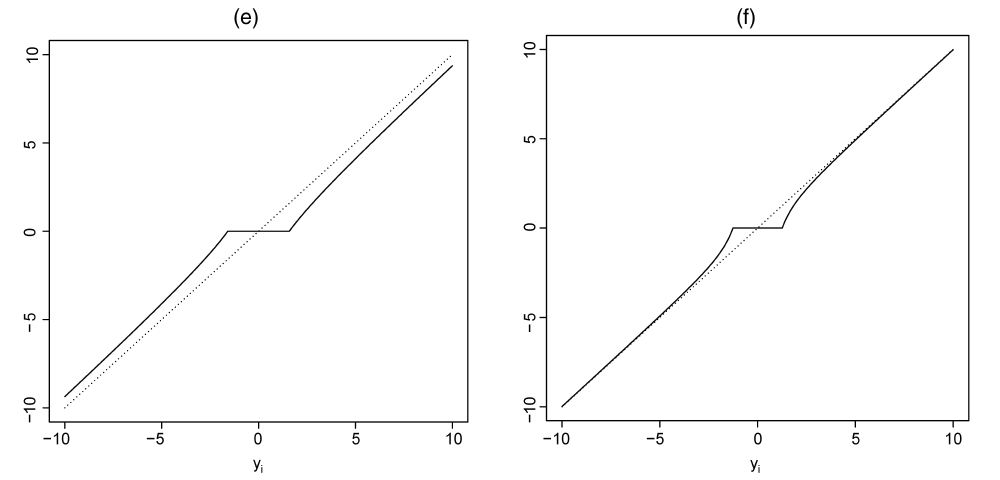
\includegraphics[width=\textwidth]{adaptive}
\begin{itemize}
\item[(e)] adaptive lasso with $\gamma = 0.5$;
\item[(f)] adaptive lasso with $\gamma = 0.2$.
\item[]
\end{itemize}
\citep[picture from][]{Zou2006}
}



%%%%%%%%%%%
\section*{Bibliography}
%%%%%%%%%%%

\frame[allowframebreaks]{\frametitle{References}
\footnotesize
\bibliographystyle{../../../../support/biometrika}
\bibliography{../../../../support/biblio}
}

\end{document}
